\documentclass[conference]{IEEEtran}
\IEEEoverridecommandlockouts
\usepackage{cite}
\usepackage{amsmath,amssymb}
\usepackage{graphicx}
\usepackage{booktabs}
\usepackage{array}
\usepackage{newtxtext,newtxmath}
\usepackage{url}
\usepackage{balance}
\graphicspath{{figures/}}

\title{Adaptive eBPF Telemetry with an Explicit Overhead Budget}
\author{\IEEEauthorblockN{Author name(s)}
\IEEEauthorblockA{Operating Systems Course\\
Institution and contact information to be completed}}

\begin{document}
\maketitle

\begin{abstract}
Kernel telemetry can clarify short-lived operating-system incidents, but continuously exporting detailed events consumes CPU and data-path capacity. This work implements an adaptive eBPF telemetry pipeline that retains a scheduler-based sentinel while controlling detailed syscall collection with three sampling modes. It compares two control mechanisms: GATE, which leaves syscall tracepoints attached and changes entry-time sampling, and SWITCH, which changes detail-link attachment state. A C/libbpf agent, target-filtered CO-RE programs, bounded event sink, deterministic CPU and tmpfs workloads, incident truth records, and a Python experiment/analysis harness form the system. We report the Linux execution evidence available in the repository: a passing privileged known-count smoke test and a four-block paired pilot comparing no detail collection with fixed 1\% sampling. The pilot estimates throughput loss of 1.85\% for CPU work and 11.21\% for I/O work; corresponding common-cutoff incident capture is 1.17\% and 1.00\%, while on-time alert recall is zero in both conditions. All pilot blocks were flagged for external CPU activity, and four blocks are below the runner's eight-block threshold for inferential budget decisions. Thus the results characterize a workload-dependent pilot trade-off, not an adaptive-policy advantage. The paper documents the implemented control path and an evidence-bounded evaluation so that subsequent fixed-frontier and adaptive experiments can be reproduced without confusing implementation checks with confirmatory findings.
\end{abstract}

\begin{IEEEkeywords}
eBPF, Linux tracing, adaptive telemetry, sampling, overhead budget, reproducible systems evaluation
\end{IEEEkeywords}

\section{Problem Definition and Objectives}
Operating-system telemetry is essential when the symptom of a failure is transient: scheduler activity, syscall behavior, or a short burst of synchronization may disappear before an operator can attach a diagnostic tool. The observer is not free. Every hook executes in kernel context, selected events consume ring-buffer and user-space work, and sustained collection can compete with the application being diagnosed. Capturing every event continuously maximizes detail but may perturb the system and overwhelm the collector; sparse sampling reduces this cost but can miss brief incidents.

This project studies the control problem stated in Assignment~4: ``observe more when needed, stay quiet when the system is healthy.'' Its research question is: \emph{at a declared application-performance budget, how do in-probe sampling and changing detail-hook attachment state affect short-incident visibility and the overhead--capture trade-off?} The implementation targets a 5\% application-throughput-loss budget and exposes LOW, MEDIUM, and HIGH collection intensities. It combines a low-cost scheduler sentinel, a trigger with hysteretic recovery and dwell time, and explicit event-loss counters. The study also distinguishes actual incident capture (received syscall pairs) from detector alert recall; these are different outcomes and neither substitutes for the other.

The engineering objectives are to implement and test the telemetry data path, compare always-attached sampling (GATE) with link switching (SWITCH), exercise controlled CPU and I/O workloads with independent incident truth, and preserve raw, validated attempts for paired analysis. The recorded pilot is a bounded fixed-rate comparison; it does not contain an adaptive-versus-fixed campaign.

\section{Related Work}
Prior work establishes that monitoring overhead can be treated as a managed resource. Software Monitoring with Controllable Overhead (SMCO) allocates runtime monitoring against a user-specified overhead target, while QVM adapts deployed defect checking under an explicit overhead manager \cite{smco,qvm}. These systems make it inappropriate to treat overhead budgets or adaptive monitoring in general as novel. Our implementation applies this broad problem framing to Linux kernel tracepoints, event transport, and an application-throughput endpoint.

Magnani \emph{et al.} present a control plane for adaptive eBPF network traffic monitoring \cite{magnani}. Their work is especially relevant because it already combines eBPF instrumentation and control-plane decisions; our study instead focuses on syscall/scheduler signals, paired CPU and cached-I/O application workloads, short synchronization incidents, and GATE-versus-SWITCH mechanisms. Naas \emph{et al.} decompose eBPF storage-I/O tracing overhead into component costs \cite{naas}; this motivates separating event selection, completion, ring reservation, sink loss, and application impact rather than reporting a single observer-cost number. Hindsight uses retroactive sampling to preserve detailed distributed traces after symptom detection \cite{hindsight}. The project’s ring buffer is only a bounded transport: it does not implement Hindsight’s historical retention abstraction.

The Linux BPF documentation describes verifier-constrained programs, maps, and user-space interaction, while libbpf documents object loading, CO-RE, and link lifecycle \cite{bpfdoc,libbpf}. These sources ground the implementation, but do not by themselves validate the measured overhead or controller behavior. Accordingly, the contribution claimed here is an implemented and reproducible comparison design with bounded Linux pilot evidence, not a first adaptive eBPF controller.

These lines of work also motivate the study's measurement choices. A single “tracing overhead” number can hide which work executes on the target path, which work scales with selected event rate, and which work occurs in the collector. The project therefore counts syscall eligibility and selection before export and records kernel reservation, completion, collector receipt, and sink outcomes separately. Similarly, adaptive monitoring should be compared against fixed policies under matched workload schedules: an adaptive controller can appear efficient simply because it sees fewer events, or appear accurate because its signal is derived from incident labels. Here the live controller receives target identifiers and prior sentinel observations, while experiment truth and application progress are recorded on separate paths. This separation is a design property; its empirical performance still depends on calibration and evaluation.

\section{System and Methodology}
\subsection{Architecture and data path}
Fig.~\ref{fig:architecture} shows the measured pipeline. A scheduler tracepoint increments a per-CPU rotating bin only when either side of a context switch belongs to a frozen target set. The user-space agent reads closed bins with a safety lag and marks torn snapshots, overwritten generations, or retention overruns as sensor gaps. In parallel, detailed syscall tracepoints use a target-TID map and allowlist for \texttt{pread64}, \texttt{futex}, \texttt{sched\_yield}, and \texttt{clock\_nanosleep}. At entry, the program samples using a generation/threshold configuration word and stores selected-call state in an in-flight map; the exit program completes that original selection even if the mode has since changed.

The sentinel uses 2,048 per-CPU bins of 5\,ms each and a 10\,ms read lag. Detailed records are 64 bytes; the collector wraps records in a block-checksummed 72-byte transport stride. The 8\,MiB BPF ring and bounded 8\,MiB writer queue have distinct reservation and sink-drop counters. The agent uses \texttt{epoll}, \texttt{timerfd}, and \texttt{signalfd}, and writes to bounded tmpfs staging. These mechanisms keep control, collection, and disk work explicit in the implementation.

\begin{figure}[t]
\centering
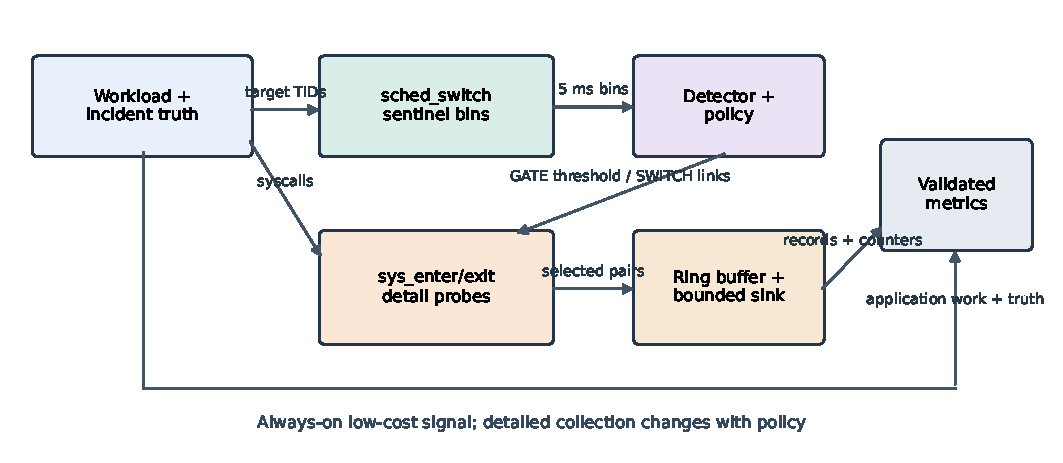
\includegraphics[width=\columnwidth]{architecture.pdf}
\caption{Implemented data path. The sentinel remains active across modes; detailed events are sampled and exported only after target and syscall filtering.}
\label{fig:architecture}
\end{figure}

\subsection{Modes and control}
LOW selects no detailed entries; MEDIUM selects 10\%; HIGH selects all eligible entries. A separate fixed 1\% policy (\texttt{FIX\_Q01}) is used for the recorded pilot. GATE keeps both syscall tracepoints attached and publishes a new sampling threshold. SWITCH attaches exit then entry with selection disabled before publishing a threshold; on a transition to LOW it disables selection, detaches entry, drains exits for at most 20\,ms, then detaches exit and classifies unresolved in-flight entries.

The detector computes the maximum standardized deviation of \(\log(1+x)\) over newly closed valid sentinel bins. Its median, robust scale (floor 0.10), threshold, and context/action cost bounds are configuration/calibration inputs, not values inferred from incident truth. The policy escalates to MEDIUM or HIGH at score thresholds, steps down after sustained quiet, uses a 500\,ms recovery interval and 250\,ms dwell by default, and requests LOW on a sensor gap. The optional supervisor constrains the requested mode using past sentinel rate and application-core utilization. Neither scheduled incident labels nor throughput measurements are supplied to the live detector.

\subsection{Signal integrity and transition accounting}
The sentinel is a per-CPU array of 2,048 rotating bins. A bin stores its epoch, count, and sequence field; the single per-CPU scheduler-switch writer brackets updates with sequence changes. The reader accepts a zero only when the requested epoch is known to have been overwritten by a newer generation or is explicitly empty. An odd sequence, newer-than-requested generation, or retention overrun is marked as a gap rather than interpreted as a quiet interval. This distinction matters to recovery: missing sensor data requests LOW and cannot accumulate evidence for de-escalation.

The detail program first checks target TID membership and a syscall allowlist. It tracks selected calls in a bounded in-flight map; the entry records syscall identity, generation, timestamp, CPU, per-target sequence, and attachment epoch. The exit handler validates the syscall identity, removes the in-flight value, and either records an explicit completion failure or emits a fixed event. Thus mode changes do not retroactively alter whether a call selected at entry is completed. A 64-bit generation/threshold word permits the agent to publish a coherent sampling configuration on the supported x86-64 target. Because sampling uses the kernel PRNG, workload seeds reproduce workload schedules, not individual sampling draws.

The agent separates instrumentation and collection outcomes in its counters. Eligible and rejected entries quantify sampling; selected, completed, emitted, and consumed events describe pipeline progress; ring reservation failures, queue/sink drops, abandoned in-flight calls, and undrained events are distinct terminal categories. A block-checksummed staging format is restored and validated after measurement. The application impact metric uses completed benchmark work; agent process samples and host CPU records are also retained, but do not by themselves identify total BPF execution cost in target context.

\subsection{Workload and experiment design}
The CPU workload runs two pinned, deterministic checksum-producing workers. The I/O workload performs explicit \texttt{pread64} calls against a prefaulted 64\,MiB tmpfs working set per worker. The full protocol supports low/high background load, workload drift, futex incidents of multiple durations, an unseen CPU-contention incident, and seven policies: NONE, SENT, fixed LOW/MEDIUM/HIGH, ADAPT\_GATE, and ADAPT\_SWITCH. The frozen design draft describes 56 primary cells and 12 paired blocks per scenario (672 trials); these are design parameters, not completed trial counts.

The evidence reported here comes from the immutable run set \texttt{bounded-q01-4blocks-20261114-001}. Its execution config uses a 5\,s warmup, 30\,s measurement, one jittered 10\,ms futex episode, low background, no drift, and four randomized paired blocks for each workload. The only compared policies are NONE and FIX\_Q01, yielding 16 valid attempts. Every attempt was retained with the preregistered \texttt{external\_cpu\_above\_threshold} noise warning.

\subsection{Pairing and measurement boundaries}
Within each workload, NONE and FIX\_Q01 runs share the block's workload and incident seeds, while policy order is randomized. The run harness waits for stable target TIDs, uses fresh owned agent/workload processes, and records the intended schedule and actual incident/helper boundaries independently of the observer. The 30\,s measured interval follows warmup and is followed by drain and cooldown; records are sealed with a checksum inventory. This pairing controls scheduled work, but cannot remove changing host interference, which is why the external-CPU warning remains part of interpretation.

Application progress is published periodically as cumulative completed work and interpolated at measured phase boundaries. The maximum bracket interval in the saved pilot is approximately 100\,ms, which is coarse relative to a 10\,ms incident. Consequently, the throughput endpoint is useful for the 30\,s application interval, but the boundary resolution does not support fine-grained claims about the precise cost or timing of a single brief incident. The report does not reinterpret work-unit duration histograms as application request latency.

\subsection{Planned primary design and executed pilot}
Table~\ref{tab:scope} distinguishes the planned matrix from the evidence actually analyzed. The primary protocol crosses seven policies with two workload families, two background levels, and two drift conditions, yielding 56 cells. Twelve randomized complete blocks per scenario are the initial target, with an adaptive precision rule permitting more blocks up to the configured cap. The planned primary execution uses 30\,s warmup, 240\,s measurement, up to 5\,s drain, and at least 15\,s cooldown. The existing pilot instead uses shorter timing, one low-background/no-drift condition, and four blocks per application family.

\begin{table}[t]
\caption{Planned primary matrix versus analyzed pilot}
\label{tab:scope}
\centering
\scriptsize
\setlength{\tabcolsep}{2pt}
\begin{tabular}{@{}p{0.72in}p{1.35in}p{1.15in}@{}}
\toprule
Factor & Planned primary design & Recorded pilot\\
\midrule
Policies & NONE, SENT, fixed LOW/MED/HIGH, ADAPT\_GATE, ADAPT\_SWITCH & NONE, FIX\_Q01\\
Workload & CPU and I/O & CPU and I/O\\
Background & Low and high & Low only\\
Drift & Absent and present & Absent\\
Blocks & 12 initially; precision rule may increase & 4 paired per workload\\
Timing & 30\,s warmup; 240\,s measured & 5\,s warmup; 30\,s measured\\
Primary volume & 56 cells; 672 initial trials & 16 attempts\\
\bottomrule
\end{tabular}
\end{table}

This distinction is important for interpreting scope: planned factors show what the harness can schedule, not what the saved data cover. The pilot has an actual 10\,ms futex episode, but it does not include the planned incident-duration ladder, high-load condition, drift transition, or adaptive mechanisms. Calibration and pilot data remain separate from any future confirmatory population; the source protocol also requires independent normal training/validation before detector thresholds can be considered frozen.

\subsection{Metrics and analysis}
For each block, application impact is \(1-\exp(\overline{\log(Q_{\mathrm{policy}}/Q_{\mathrm{NONE}})})\), where \(Q\) is completed application work per measured interval. The runner reports a 10,000-draw whole-block bootstrap interval and a one-sided 95\% budget bound. At budget \(B=0.05\), its compliance decision is compliant, violating, or inconclusive. The runner explicitly marks fewer than eight independent blocks as underpowered; therefore the pilot's budget status is inconclusive even where the point estimate exceeds 5\%.

Incident capture is the fraction of independently counted helper syscall pairs received by the collector by the common cutoff. Alert recall is calculated separately from detector alerts matched chronologically to actual incident intervals. Event counters separately account for eligible, selected, rejected, completed, emitted, ring-reservation failure, sink drop, abandoned, and undrained records. Negative throughput-loss estimates are retained by the analysis rather than clipped.

For alert metrics, actual onset/end timestamps define the matching window; chronological one-to-one matching prevents one alert from satisfying multiple incidents. On-time recall is reported separately from post-incident detection, and a missing alert remains a miss rather than being dropped from delay summaries. For syscall capture, the denominator is the independent helper-call truth ledger and the numerator is correctly received pairs before the common cutoff. The analysis also retains capture thresholds (one and ten useful pairs) and policy mode occupancy/transitions when those outcomes are available. These distinct estimands avoid equating a sampled syscall record with a detector success.

\section{Implementation and Linux Validation}
The kernel programs are C eBPF CO-RE sources under \texttt{src/bpf/}; the collector and workload generators are C; orchestration, schemas, validation, and statistics are Python. The recorded Linux host is Ubuntu 26.04 LTS, x86-64, kernel \texttt{7.0.0-31-generic}, with 20 logical CPUs and approximately 14.5\,GiB RAM. The recorded toolchain includes Python 3.14.4, Clang 18.1.8, GCC 15.2.0, GNU Make 4.4.1, and bpftool 7.7.0. The agent build uses the pinned libbpf 1.5.1 source build; the installed bpftool reports its own libbpf 1.7 runtime.

The privileged smoke test passed on 2026-11-14. For 2,000 eligible entries at full selection, the ledger recorded 2,000 selected, completed, emitted, consumed, and written events; ring-reservation failures, sink drops, abandoned calls, and undrained events were zero. The low-mode known-count check selected zero of 2,000 eligible entries, and the sentinel-only check emitted no detailed records. These checks establish basic loading, counting, transport, and cleanup behavior on the recorded host; they are not a performance campaign.

\section{Results}
Table~\ref{tab:pilot} reports the actual paired pilot summaries. FIX\_Q01 denotes entry sampling at probability 0.01 against the paired NONE baseline. The confidence intervals are the runner's two-sided 95\% whole-block bootstrap intervals. All four blocks per workload are flagged for external CPU activity; estimates should consequently be read as exploratory observations, not clean-host causal estimates.

\begin{table}[t]
\caption{Four-block Linux pilot: FIX\_Q01 versus NONE}
\label{tab:pilot}
\centering
\scriptsize
\begin{tabular}{@{}lccc@{}}
\toprule
Workload & Throughput loss (95\% CI) & Capture (95\% CI) & On-time recall\\
\midrule
CPU & \shortstack{1.85\%\\{}[--0.63, 5.60]\%} & \shortstack{1.17\%\\{}[1.02, 1.35]\%} & 0\%\\
I/O & \shortstack{11.21\%\\{}[10.85, 11.46]\%} & \shortstack{1.00\%\\{}[0.88, 1.16]\%} & 0\%\\
\bottomrule
\end{tabular}
\end{table}

The I/O point estimate is 11.21\% throughput loss, compared with 1.85\% for CPU work. This contrast is consistent with the very different eligible syscall volumes and shows why a fixed sampling probability does not imply a workload-independent application cost. Neither policy/workload combination demonstrated on-time detector recall in this run set. The captured helper-pair fraction is near the configured sampling probability, but it is not evidence that the anomaly detector identified the incidents.

For context, summing the four FIX\_Q01 attempt ledgers per workload gives 24,207 eligible and 280 selected entries for CPU, and 103,902,521 eligible and 1,038,842 selected entries for I/O. Both totals recorded zero ring-reservation failures and zero sink drops; one in-flight event was classified abandoned per workload set. Thus low exported volume arose primarily from sampling, not an observed transport overflow. The event-ledger totals and the capture fraction have different denominators and should not be interchanged.

\begin{table}[t]
\caption{Summed FIX\_Q01 event ledger across four attempts}
\label{tab:events}
\centering
\scriptsize
\begin{tabular}{@{}lrrr@{}}
\toprule
Workload & Eligible & Selected & Completed/received\\
\midrule
CPU & 24,207 & 280 & 279\\
I/O & 103,902,521 & 1,038,842 & 1,038,841\\
\bottomrule
\end{tabular}
\end{table}

The selected-to-eligible ratios derived from these totals are 1.16\% for CPU and approximately 1.00\% for I/O. The one-call difference between selected and completed/received in each workload is consistent with the single in-flight event classified abandoned in its four-run set; it is not a ring-buffer or sink loss. The I/O stream generated approximately 866,000 eligible entries per second in aggregate across its two-minute measured exposure, so the 1\% policy still passed roughly 8,700 selected calls per second to the collector. This illustrates why the sampling probability alone is not a sufficient description of absolute event volume or user-space work.

\subsection{Overhead budget as an evaluation endpoint}
The declared 5\% target is defined on paired application throughput over a measured interval, not as a hard per-tick CPU ceiling. This makes the budget interpretable to an operator: a monitoring configuration is judged by the application work it displaces relative to the same seeded no-detail baseline. The controller's optional resource supervisor is a separate mechanism: it constrains mode requests using calibrated context/action bounds and recent load, but it does not observe throughput during a trial. Model uncertainty and unresolved transition costs are retained as uncertainty rather than converted to zero cost.

The pilot demonstrates why an explicit denominator and paired baseline matter. CPU work completes substantially more checksum batches per interval than the I/O workload completes reads, and the I/O application produces orders of magnitude more eligible syscalls. A fixed 1\% entry probability therefore yields comparable fractions of eligible entries but very different absolute event rates and application impacts. The pilot has no NONE/SENT-to-fixed-high frontier and no adaptive policy, so it cannot identify the best point under the budget. It does, however, motivate conditioning cost estimates on workload and mode, as already represented by the project's calibration and context/action cost tables.

The confidence-interval rule also prevents a favorable point estimate from being treated as budget compliance. Compliance requires a sufficiently supported one-sided upper bound at or below 5\%; violation requires the corresponding lower-bound evidence above 5\%. With four blocks, the runner deliberately returns inconclusive. This is conservative but transparent: the interval is shown, all four paired values remain available, and no significance statement is inferred from event counts or within-run samples.

\begin{figure}[t]
\centering
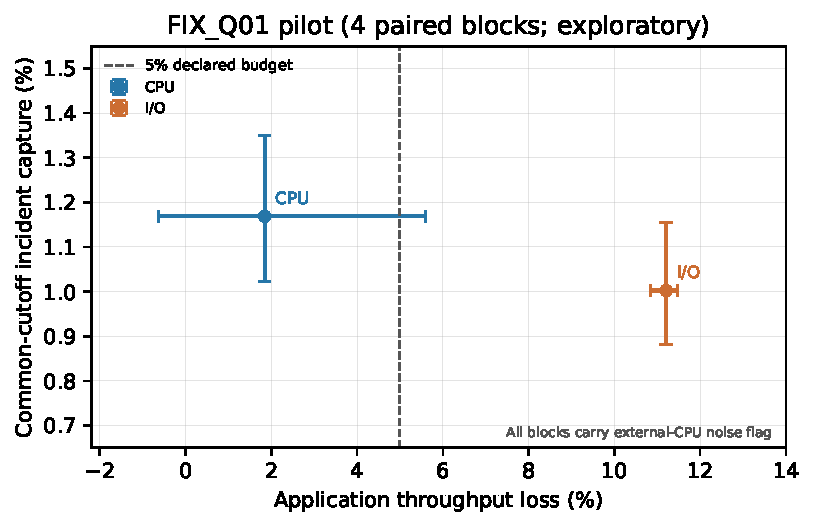
\includegraphics[width=\columnwidth]{pilot_frontier.pdf}
\caption{Measured pilot throughput-loss and common-cutoff-capture estimates. Error bars show 95\% block-bootstrap intervals; the dashed line is the declared 5\% throughput budget. All four blocks in each condition have an external-CPU noise warning.}
\label{fig:frontier}
\end{figure}

The CPU interval spans zero and the declared budget, while the I/O interval lies above the budget value. Nonetheless, the analysis marks both formal compliance classifications inconclusive because \(n=4\) is below its preregistered minimum for inferential decisions. This distinction preserves the observed estimate without converting a small, noisy pilot into a budget claim. The fixed 1\% pilot also does not test the central adaptive-policy hypothesis, compare the complete fixed-rate frontier, or quantify adaptation delay and mode stability.

The zeros in on-time alert recall should be read alongside the positive, near-1\% pair capture. The collector did receive some syscall detail, but a sampled helper event is not itself an anomaly alert: the alert path is driven by the scheduler sentinel and calibrated score. In these runs the detector did not produce an on-time alert for the single scheduled incident. The present data do not isolate whether that outcome arose from incident duration, signal separation, threshold calibration, or host interference, so assigning a cause would go beyond the records.

\section{Discussion and Limitations}
The main empirical observation is workload dependence: the same fixed sampling probability was associated with materially different application-throughput impacts in the two measured workloads. The event ledger narrows interpretation by showing no ring or sink drops in these pilot attempts. The passing known-count smoke further establishes that the instrumented high-mode path can deliver a controlled event count on the recorded host.

There are important boundaries. The pilot has four paired blocks and every block is noise-flagged; its bootstrap intervals are descriptive and the runner labels them underpowered. It has only one short incident per trial, low background, no drift, and no adaptive policy. The 1\% policy is not the 10\% MEDIUM mode. No result here establishes that ADAPT\_GATE or ADAPT\_SWITCH meets the 5\% budget or improves detection per unit overhead. Per-process resource samples and host CPU records are preserved, but the reported endpoint is paired application throughput, not an isolated causal estimate of total BPF CPU cost. Workload boundary interpolation is about 100\,ms in the recorded attempts, limiting fine-grained timing interpretations.

The host noise flag does not invalidate the attempt's internal accounting, but it does weaken attribution of throughput differences to telemetry alone. Four blocks also yield a discrete, broad bootstrap distribution; reporting hundredths of a percent in a point estimate does not imply equivalent precision. A clean-host sensitivity run and more independent blocks are necessary before drawing a budget conclusion. The current I/O throughput point estimate is above 5\%, but the declared analysis rule remains inconclusive at this sample size rather than converting it into a formal violation.

The implementation accounts for specific lifecycle races and loss channels, but the known-count smoke is not a substitute for longer concurrency, failure-injection, and full-matrix acceptance tests. The saved pilot does not include drift, high background, the duration ladder, hysteresis/dwell ablations, or a separately powered false-alarm study. Claims are limited to this host, kernel, workload, and pilot configuration. The next comparison should pair the complete fixed sampling frontier with both adaptive mechanisms under the same randomized schedules, report application and observer resource costs separately, and retain noise-flagged or failed attempts in the evidence record.

The workload itself is controlled but synthetic at the application layer. The I/O case uses a warm tmpfs working set and thus exercises syscall/tracing behavior without representing physical-device latency or a production storage stack. The futex helper pair creates repeatable synchronization activity and independent call-count truth, but it is not a general model of application incidents. The fixed worker placement, single host, and kernel build likewise bound transferability. These choices support reproducible within-host mechanism comparison; they do not justify extrapolation to different kernels, storage devices, or service request distributions.

There is also a measurement-boundary limitation. The primary throughput samples are cumulative counters interpolated around phase boundaries, with approximately 100\,ms maximum bracketing in the pilot. That resolution is appropriate for a 30\,s interval-level effect, but cannot resolve a 10\,ms event's exact onset cost. In future duration-sensitivity results, incident truth timestamps and call capture should therefore carry the fine-grained timing claims, while application-throughput differences should remain attached to their longer measurement interval.

\section{Conclusion}
We implemented a Linux eBPF observability system with a persistent scheduler sentinel, sampled syscall detail, three telemetry modes, GATE and SWITCH transition mechanisms, explicit event accounting, controlled workloads, and a reproducible paired-run harness. The actual privileged smoke test delivered all expected high-mode records without ring or sink loss. The four-block fixed 1\% pilot measured substantially different throughput impact for CPU and I/O workloads and approximately 1\% common-cutoff incident capture in both, with zero on-time alerts. Because the pilot is small, noise-flagged, and does not contain adaptive policies, it does not establish adaptive superiority or budget compliance. It does provide concrete Linux measurements and a traceable base for the planned fixed-frontier and adaptive comparisons.

\balance
\bibliographystyle{IEEEtran}
\bibliography{references}
\end{document}
